%
% File naaclhlt2018.tex
%
%% Based on the style files for NAACL-HLT 2018, which were
%% Based on the style files for ACL-2015, with some improvements
%%  taken from the NAACL-2016 style
%% Based on the style files for ACL-2014, which were, in turn,
%% based on ACL-2013, ACL-2012, ACL-2011, ACL-2010, ACL-IJCNLP-2009,
%% EACL-2009, IJCNLP-2008...
%% Based on the style files for EACL 2006 by 
%%e.agirre@ehu.es or Sergi.Balari@uab.es
%% and that of ACL 08 by Joakim Nivre and Noah Smith

\documentclass[11pt,a4paper]{article}
\usepackage[hyperref]{naaclhlt2018}
\usepackage{times}
\usepackage{latexsym}

\usepackage{url}

%%%LK: I added the lines below:
\usepackage{rotating}
\usepackage{tikz}
\usetikzlibrary{shapes,arrows}
\usepackage{graphicx}
\usepackage{tikz-dependency}
\usepackage{natbib}
\usepackage{amsmath}
\DeclareMathOperator*{\argmax}{arg\,max}
\DeclareMathOperator*{\argmin}{arg\,min}
\usepackage{tikz-qtree}
\usepackage{multirow}
\usepackage{rotating}
\usepackage{booktabs}
%% MD: some versions of latex need this package to be loaded last
%\usepackage{gb4e}
%%%LK: I added the lines above

%\aclfinalcopy % Uncomment this line for the final submission
%\def\aclpaperid{***} %  Enter the acl Paper ID here

%\setlength\titlebox{5cm}
% You can expand the titlebox if you need extra space
% to show all the authors. Please do not make the titlebox
% smaller than 5cm (the original size); we will check this
% in the camera-ready version and ask you to change it back.

\newcommand{\feat}[1]{\texttt{#1}}
\newcommand{\md}[1]{\marginpar{\scriptsize MD: #1}}
\newcommand{\lk}[1]{\marginpar{\scriptsize LK: #1}}
% for removing all marginpars ==> good for final submission! %%nice trick!
%%\renewcommand{\marginpar}[1]{}

\newcommand\BibTeX{B{\sc ib}\TeX}
\title{Annotating Picture Description Task Responses for Content Analysis}

\author{Levi King \\
  Indiana University \\
  {\tt leviking@indiana.edu} \\\And
  Markus Dickinson \\
  Indiana University \\
  {\tt md7@indiana.edu} \\}

\date{}

\begin{document}
\maketitle
\begin{abstract}
Given that all users of a language can be creative in their language usage, the overarching goal of this work is to investigate issues of variability and acceptability in written text, for both non-native speakers (NNSs) and native speakers (NSs).  We control for meaning by collecting a dataset of picture description task (PDT) responses from a number of NSs and NNSs, and we annotate a handful of dimensions, to capture the multifaceted ways in which responses can vary and can be acceptable.  Outlining the decisions to be made highlights questions needing to be addressed by anyone working with learner language properties such as variability, acceptability and native-likeness.  We find reliable inter-annotator agreement, though areas of disagreement highlight difficult areas for establishing a link between form and meaning.
\end{abstract}

\section{Introduction}

% motivations
% \begin{itemize}
% \item why are we doing what we're doing?
% \item why should someone care?
% \end{itemize}

% Who should care:
% \begin{itemize}
% \item Everyone working with learner data needs to account for its variability
% \item Anyone who wants to deal with acceptability needs to have a definition of what acceptability means
% \end{itemize}

% Our work:
% \begin{itemize}
% \item provides dimensions of acceptability
% \item variability is based on form-meaning matches, and to understand it means knowing what the person intended the meaning to be.  To study variability, we need to control for meaning.  (trick: we don't really know intention, but we do know what the acceptable meaning is for a picture.)
% \end{itemize}

%%Chapter 3, �Special Problems of Language Learners,� outlines the special properties of learner errors, which are often very different from the errors that native speakers make because of the influence of the learner�s native language. We go into some detail presenting three common errors in learner language: those involving prepositions, articles, and collocations.

The (written) data of second language learners poses many challenges, whether it is being analyzed for grammatical errors \citep{leacock:ea:14}, for linguistic patterns \citep{kyle2015automatically}, for content analysis \citep{weigle2013english}, or for interactions with intelligent computer-assisted language learning (ICALL) systems \citep{amaral:meurers:user:07}. One of the core issues in doing anything with learner data is the inherent amount of variability in how linguistic forms are used to convey meaning \citep[cf., e.g.,][]{Meurers.Dickinson-17}. It may indeed seem like learners can use an infinite variety of forms to express a particular meaning. 
%
But the question of how large the problem of variability is for computational processing has rarely been investigated. More specifically, within the space of possible language productions, there is the question of determining which variations are acceptable ones for a given setting.
%Taking this as an overarching question, 

Our overarching goal is to investigate these questions of variability and acceptability, both for non-native speakers (NNSs) and native speakers (NSs), given that all users of a language can be creative in their language usage.
%
To that end---and taking \textit{variability} to concern different mappings between linguistic form and its meaning---in this paper we control for meaning by collecting a dataset of picture description task (PDT) responses from a number of NSs and NNSs, and we annotate a handful of dimensions, thereby capturing the multifaceted ways in which responses can vary and can be acceptable or unacceptable. We call this the SAILS Corpus, for \textit{semantic analysis of image-based learner sentences}. \lk{We should declare the name, I think. How about this?} Outlining the decisions to be made highlights questions needing to be addressed by anyone working with learner language properties such as variability, acceptability and native-likeness.

% \begin{itemize}
% \item Background, purpose of the corpus; (variability within NS and NNS groups; and these groups vary from each other?)
% \end{itemize}

Given the form-meaning aspect of variability, we are interested in how variable linguistic behavior is \emph{for the same content}, both within and among NSs and NNSs.  There is a long-standing notion that systems processing learner data would be wise to constrain the data in some way \citep[e.g.,][]{heift:schulze:07, somasundaran:chodorow:14, somasundaran:ea:15}, but we do not know how much constraint is needed---or whether we sacrifice the possibility of observing particular learner behavior for the sake of a constraint---without knowing more about the ways in which variation happens \citep[cf., in particular,][]{bailey:meurers:08}.  

Using responses to PDT stimuli ensures that respondents are discussing the same content.  In further annotating multiple dimensions of these PDT responses, not only are we able to see how variable they are, but we are able to get a better handle on what could make them more appropriate for different purposes.  For example, knowing that a person has gotten the main content of a picture correct, while adding information not present in the picture, may be treated differently than one who has made no such inferences but seems to be addressing a question about a different person in the picture (see section~\ref{sec:scheme}).  The acceptability of a response is thus taken as a function of several interacting features, most of which relate the text to the known semantic content.  Relating to known content is distinct from typical grammatical error correction (GEC) \citep{leacock:ea:14} and from more linguistically driven work such as parsing \citep[e.g.,][]{cahill-et-al:14, ragheb:dickinson:14a}, but providing the dimensions of acceptability and elucidating how they are applied provides insight for any enterprise desiring to connect learner text with semantic content, in addition to unpacking the sources of variation and of difficulty in processing a range of learner data.

%nature of variation more generally.

% Enterprises such as ICALL and grammatical error correction (GEC)
% %, under their different conditions, 
% could benefit by knowing more about the sources of difficulty in processing the range of learner data they do.

% \begin{itemize}
% % \item Motivate this for people who don't do this kind of work; measuring 'goodness' of responses; decomposing them into features; (this is not like grammatical error detection or parsing work); Getting a handle on variability, especially under different circumstances; is a response 'native-like'? in what ways (by which features?); breaking variability down into our features;
% \item Anyone working on the automatic processing of learner data can benefit from better understanding the range of variability, and anyone who wants to speak of learner data as diverging from native data needs to qualify the exact nature of that divergence.
% \item Our work:
%   \begin{itemize}
%   \item provides dimensions of acceptability
%   \item variability is based on form-meaning matches, and to understand it means knowing what the person intended the meaning to be.  To study variability, we need to control for meaning.  (trick: we don't really know intention, but we do know what the acceptable meaning is for a picture.)
%   \end{itemize}
% \item Cite previous work:
%   \begin{itemize}
%   \item ours \citep{king:dickinson:13} 
%   \item and others' \citep{somasundaran:ea:15}
%   \end{itemize}
% \end{itemize}

Taking a cue from \citet{king:dickinson:13}, in section~\ref{sec:pdt} we outline the picture description task (PDT) we use, designing items that elicit specific types of linguistic behavior.  Section~\ref{sec:scheme} outlines the annotation, specifically tackling the five-dimensional scheme; inter-anntotator agreement results are provided in section~\ref{sec:agreement}.  While agreement seems reliable, highlighting areas of disagreement showcases difficult areas for establishing a link between form and meaning \citep[cf., e.g.,][]{Meurers.Dickinson-17}.

\section{Picture Description Task}
\label{sec:pdt}

\subsection{PDT Stimuli}

The PDT is built around 30 cartoon-like vector graphics, or \textbf{items}. The images were modified to remove any non-essential detail or background; some examples are in Table~\ref{tab:test-sample-items}. To factor out the influence of previous linguistic context, images are devoid of any text or symbols, with the exceptions of two images containing numerals, two with music notes, and one with a question mark. Each image depicts an ongoing or imminent action, performed by a person or an animal. The images are divided evenly into canonically intransitive, transitive and ditransitive actions. 

Two main versions of the PDT were used. In each version, the first half contains \textbf{targeted} items, where questions take the form of \textit{What is $<$subject$>$ doing?}, with the subject provided (e.g., \textit{the boy}, \textit{the bird}). The second half contains \textbf{untargeted} items, where the question is, \textit{What is happening?}. Collecting both versions allows one to examine response variation with and without a subject constraint, thereby informing approaches to task design and automatic content assessment \citep{foster2009native, cho2013investigating}. Roughly equal numbers of targeted and untargeted \textbf{responses} were collected for each item.

Each half (targeted and untargeted) is introduced with instructions, including an example item with sample responses. The instructions ask participants to focus on the main event depicted in the image and for each response to be one complete sentence. The PDT was presented as an online survey, and all participants typed their responses. Participants were instructed not to use any reference materials, but were permitted to use browser-based spell checking.

%% LK NTS:
%%intransitive is I30 (woman is running)
%%transitive is I29 (woman is hugging dog)
%%ditransitive is I28 (man is giving directions)
\begin{table}[htb!]
%\begin{table}[t!] This line is giving me trouble when I go to typeset
\begin{center}
\begin{tabular}{|l|c|c|}
\hline
\multicolumn{3}{|c|}{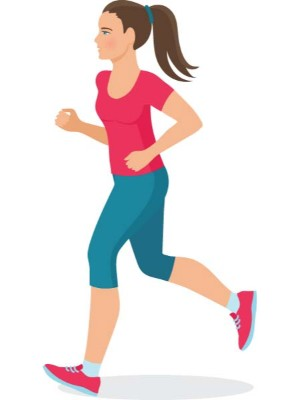
\includegraphics[width=0.35\columnwidth]{figures/I30.jpg}} \\
\hline
%\multicolumn{3}{|l|}{What is the woman doing? [Intransitive]} \\
What is the woman doing? [Intrans.] & A1 & A2 \\
\hline
The woman is running. & 1 & 1 \\
\hline
She is wearing a red shirt. & 0 & 0 \\
\hline
Trying to run from her bad decisions & 1 & 0 \\
\hline
\hline
\multicolumn{3}{|c|}{
\includegraphics[width=0.35\columnwidth]{figures/I29.jpg}} \\
\hline
What is the woman doing? [Trans.] & A1 & A2 \\
\hline
Holding a puppy \& looks happy & 1 & 1 \\
\hline
She is happy with the dog. & 0 & 0 \\
\hline
The lady loves her dog. & 1 & 0 \\
\hline
\hline
\multicolumn{3}{|c|}{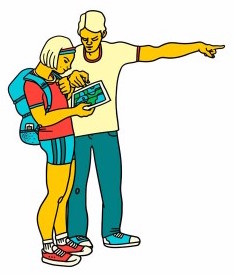
\includegraphics[width=0.5\columnwidth]{figures/I28.jpg}} \\
\hline
What is the man doing? [Ditrans.] & A1 & A2 \\
\hline
giving directions to a woman. & 1 & 1 \\
\hline
The man is reading a map. & 0 & 0 \\
\hline
The man is is telling her where to go & 1 & 0 \\
\hline
\end{tabular}
\caption{\label{tab:test-sample-items} Test sample items and example responses with Core Event annotations from Annotators 1 and 2.}
\end{center}
\end{table}


\subsection{Data Collection}

Responses were collected from 499 participants. Of these, 141 were NNSs, recruited from intermediate and advanced writing courses for English as a Second Language students attending a large public university in the US. These participants were native speakers of Mandarin Chinese (125), Korean (4), Burmese (3), Hindi (2), and one native speaker each of Arabic, Indonesian Bahasa, German, Gujarati, Spanish, Thai and Vietnamese. 

Of the 358 NS participants, 29 were personally known by the researchers. Responses from the remaining 329 NSs were purchased via an online survey platform where participants earn credits they can redeem for gift cards and prizes. Due to length restrictions for purchased surveys, these NSs each completed only half of the task, so their data is equivalent to 164.5 full participants.

In previous similar work \citep{king:dickinson:13,king:dickinson:16}, NSs were found to produce less variation than NNSs. Many NSs provided identical responses or ones very similar to the most canonical way of expressing the main action. One purpose of gathering the data is to be able to assess NNS response content by comparing it against the NS responses; thus, NSs were asked to provide two non-identical responses, in the hopes that this would result in more examples of native-like responses for the NNS responses to compare against.

%% LK NTS:
%%intransitive is I30 (woman is running)
%%transitive is I29 (woman is hugging dog)
%%ditransitive is I28 (man is giving directions)
\begin{table}[htb!]
\begin{center}
\begin{tabular}{|l||l|l||l|l|}
\hline
 & \multicolumn{2}{|c||}{Targeted} & \multicolumn{2}{|c|}{Untargeted} \\
\hline
 Set & NS & NNS & NS & NNS \\
\hline
\hline
Intrans & 0.628 & 0.381 & 0.782 & 0.492 \\
\hline
Trans & 0.752 & 0.655 & 0.859 & 0.779 \\ %%LK: Yes, 0.949 is correct in both cases here
\hline
Ditrans & 0.835 & 0.817 & 0.942 & 0.936 \\ 
\hline
\end{tabular}
\caption{\label{tab:ttr} NS and NNS type-to-token ratios (TTR) for complete responses (not words), for all the data. }
\end{center}
\end{table}

To examine the degree of variation among the NS and NNS groups in the current study, type-to-token ratios (TTR) were calculated on the response level (ignoring case and final punctuation) for the entire set of items, shown in Table~\ref{tab:ttr}. For each data point in the table, the corpus contains roughly 150 NS responses and 70 NNS responses. To control for this imbalance and its effect on the likelihood of seeing new responses, the TTR was calculated for each item based on a random sample of 50 responses.  Specifically, we randomly sampled 50 responses, calculated the TTR, and averaged them. 
%Then, for intransitives, transitives and ditransitives, as shown, the TTR was calculated as the average TTR of the ten items in each set. 
The scores in in Table~\ref{tab:ttr} show that, in all cases, the NS set shows a greater degree of response variation, meaning that asking for two responses is an effective way of collecting a broader range of NS responses.

The ratios show the direct relationship between the complexity of the event portrayed (represented here as intransitive, transitive and ditransitive) and the degree of variation elicited. In all cases, TTR increases with this complexity. Interestingly, this trend seems more pronounced in the NNS responses; in the targeted NNS responses, the TTRs for intransitive and ditransitive items are 0.381 and 0.817, respectively, compared to 0.628 and 0.835 for NS responses. The ratios also show that in all cases, variation is greater for untargeted items than it is for targeted items. In other words, asking about a particular subject in the prompt question does constrain the variety of responses.


\section{Annotation scheme}
\label{sec:scheme}
The data were annotated with the aim of providing information that would be useful for the automatic assessment of NNS responses via comparison with NS responses.  
%A five-dimension annotation scheme was developed to capture different facets of assessment.
%
%; insights gained from the annotation, and in particular an interannotator agreement study, are covered in section~\ref{sec:agreement}.
%
The annotation scheme was developed through an iterative process of annotation, discussion and revision, with input from two annotators and multiple language professionals. The initial scheme was planned as a three-point scale, ranging from \textit{accurate and native-like} (2) to \textit{accurate but not native-like} (1) to \textit{not accurate} (0). This proved problematic, however, as \textit{accuracy} and \textit{native-likeness} could not be adequately defined and applied to the data.
%\marginpar{MD: A quick example of inadequacy would be nice here.}
For example, in the middle picture of Table~\ref{tab:test-sample-items}, it is not clear how accurate or native-like \textit{She is happy with the dog} is.  Grammatically, it is native-like, but it does not seem like an appropriate answer to the question, \textit{What is the woman doing?}

To address the specifics of appropriate answers, five binary features were eventually settled on, with each feature having some relation to the original concepts of accuracy and native-likeness. A set of annotation guidelines were produced with definitions, rules and examples for each feature. For most features, the rules for targeted and untargeted items vary slightly; the untargeted rules are generally less strict. The features and brief descriptions are listed here and discussed further in the following sections:

\begin{enumerate}
\item \textbf{Core Event}: Does the response capture the core event depicted in the image? Core events are not pre-defined but should be fairly obvious given the nature of the images. The response should link an appropriate subject to the event.  In the top picture of Table~\ref{tab:test-sample-items}, \textit{The woman is running} clearly captures the core event, while \textit{She is wearing a red shirt} is irrelevant to the event happening.
\item \textbf{Verifiability}: Does the response contain only information that is true and verifiable based on the image? Inferences should not be speculations and are allowed only when necessary and highly probable, as when describing a familial relationship between persons depicted in the image.  For example, in Table~\ref{tab:test-sample-items}, \textit{She is wearing a red shirt} conveys information that is irrelevant to the core event but is nonetheless recoverable from the image (annotation=1), while \textit{Trying to run from her bad decisions} has information that cannot be inferred from the picture.
\item \textbf{Answerhood}: Does the response make a clear attempt to answer the question? This generally requires a progressive verb. For targeted items, the subject of the question, or an appropriate pronoun, must be used as the subject of the response.  For example, \textit{The dog is happy} is answering a question other than \textit{What is the woman doing?} (Table~\ref{tab:test-sample-items}).
\item \textbf{Interpretability}: Does the response evoke a clear mental image (even if different from the item image)? Any required verb arguments must be present and unambiguous.  For example, \textit{The map is hard to read} is too vague to generate a clear mental image (see Table~\ref{tab:test-sample-items}).
\item \textbf{Grammaticality}: Is the response free from errors of spelling and grammar?  
%While the focus of GEC work, 
In our data set, this is a relatively straightforward feature to annotate (see section~\ref{sec:agreement}).
%\lk{Is it straightforward?} 

\end{enumerate}

\paragraph{Example annotations}

In Table~\ref{tab:devo-transitive}, we see example responses with all five features annotated, illustrating each feature's distinctiveness from the others.  For example, for \textit{He is eating food} one can generate a mental picture, e.g., of someone chewing (\feat{interpretability}=1), but the pizza is important to the item image (\feat{core event}=0).  As another example, \textit{He may get fat eating pizza} seems to be addressing a question about the consequences of the eating action (\feat{answerhood}=0) and talks about hypotheticals not in the picture (\feat{verifiability}=0).
%, while all other features are correct.  
Teasing apart these annotations is the focus of the next section.

\begin{table}[htb!]
%\begin{table}[t!] This line is giving me trouble when I go to typeset
\begin{center}
\begin{tabular}{|p{3.7cm}|c|c|c|c|c|}
\hline
\multicolumn{6}{|c|}{
\includegraphics[width=0.45\columnwidth]{figures/I02.jpg}} \\
\hline
%\multicolumn{3}{|l|}{What is the woman doing? [Intransitive]} \\
\textit{What is the boy doing?} & C & V & A & I & G \\
\hline
\hline
He is eating food. & 0 & 1 & 1 & 1 & 1 \\
\hline
eatting. & 0 & 1 & 1 & 1 & 0 \\
\hline
The child is about to eat pizza. & 1 & 1 & 0 & 1 & 1 \\
\hline
He may get fat eating pizza. & 1 & 0 & 0 & 1 & 1 \\
\hline
\hline
\hline
\textit{What is happening?} & C & V & A & I & G \\
\hline
\hline
Child is eating pizza. & 1 & 1 & 1 & 1 & 0 \\
\hline
Tommy is eating pizza. & 1 & 0 & 1 & 1 & 1 \\
\hline
The boy's eating his favorite food. & 0 & 0 & 1 & 0 & 1 \\
\hline
Pizza is this boy's favorite food. & 0 & 0 & 0 & 0 & 1 \\
\hline
\end{tabular}
\caption{\label{tab:devo-transitive} Targeted and untargeted sample responses from the development set transitive item, shown with adjudicated annotations for the five features: core event (\textit{C}), verifiability (\textit{V}), answerhood (\textit{A}), interpretability (\textit{I}) and grammaticality (\textit{G}).}
\end{center}
\end{table}

\section{Agreement}
\label{sec:agreement}
Two annotators participated in the annotation. Both are native speakers of (US) English, and each has several years of language teaching experience with both children and adult learners. Annotator 1 (A1) annotated the complete corpus. Annotator 2 (A2) annotated only the development set and the test set, data subsets described next.

\begin{table*}[htb!]
\begin{center}
\begin{tabular}{|l|l|l|l|l||l|l||l|}
\hline
Set	& Total	& A1Yes & A2Yes & AvgYes & Chance & Agree & Kappa \\
\hline
\hline
Intrans & 2155 & 0.863 & 0.855 & 0.859 & 0.758 & 0.978 & 0.910 \\
\hline
Trans & 2155 & 0.780 & 0.774 & 0.777 & 0.653 & 0.949 & 0.853 \\
\hline
Ditrans & 2155 & 0.812 & 0.786 & 0.799 & 0.678 & 0.924 & 0.764 \\ 
\hline
\hline
Target & 3390 & 0.829 & 0.818 & 0.824 & 0.709 & 0.949 & 0.823 \\
\hline
Untarg & 3075 & 0.806 & 0.790 & 0.798 & 0.678 & 0.952 & 0.872 \\
\hline
\hline
Core & 1293 & 0.733 & 0.717 & 0.725 & 0.601 & 0.923 & 0.808 \\
\hline
Verif & 1293 & 0.845 & 0.817 & 0.831 & 0.719 & 0.968 & 0.884 \\
\hline
Answer & 1293 & 0.834 & 0.831 & 0.833 & 0.721 & 0.982 & 0.936 \\
\hline
Interp & 1293 & 0.818 & 0.787 & 0.802 & 0.682 & 0.919 & 0.744 \\
\hline
Gramm & 1293 & 0.861 & 0.872 & 0.866 & 0.768 & 0.960 & 0.827 \\
\hline
\end{tabular}
\caption{\label{tab:agreement} Agreement scores broken down by different properties of the test set: total annotations (\textit{Total}), \textit{yes} annotations for Annotator 1 and 2 (\textit{A1Yes}, \textit{A2Yes}), average \textit{yes} annotations (\textit{AvgYes}), total expected chance agreement for \textit{yes}es and \textit{no}s (\textit{Chance}), actual raw agreement (\textit{Agree}) and Cohen's kappa (\textit{Kappa}).}
\end{center}
\end{table*}

Three items were used as a development set for creating and revising the annotation scheme. These items were also used as examples in the guidelines. They represent one intransitive, one transitive and one ditransitive item. Both annotators annotated portions of the development set multiple times throughout the process, discussing and adjudicating disagreeing annotations before moving on to the test set, which was completed without consultation between the annotators.

The test set parallels the development set and consists of one intransitive, one transitive and one ditransitive item; it is shown in Table~\ref{tab:test-sample-items}. Agreement and Cohen's kappa scores are given in Table~\ref{tab:agreement}, broken down by different criteria.  We will now walk through these results.

\subsection{Transitivity} 
\label{sec:transitivity}
Comparing the intransitive, transitive and ditransitive items reveals an association between agreement and item complexity. The highest raw agreement and Cohen's kappa scores are found with the intransitive item ($97.8\%$, $\kappa=0.910$) and the lowest with the ditransitive ($92.4\%$, $\kappa=0.764$). 

This is as expected, as ditransitive sentences are longer and have more verbal arguments, making for more opportunities for responses to vary (see Table~\ref{tab:ttr}), and thus more opportunities for annotators to disagree on a response. This trend also matches annotator feedback: both ranked the ditransitive item as the most difficult to annotate, for all features, and the intransitive as the easiest.

\subsection{Targeting} 
\label{sec:prompts}
Grouping the annotations into targeted and untargeted sets, the raw agreement scores are comparable ($94.9\%$ vs. $95.2\%$). However, despite a greater degree of response variation, the untargeted group has a higher kappa score ($0.872$ vs. $0.823$).
%
%\md{Still thinking through the connection with AvgYes scores ...}
%
When asked to compare the annotations, A2 noted that targeted responses require more concentration and closer consultation of the guidelines. For example, \feat{answerhood} does not allow for targeted responses to modify the subject provided in the question in any way, whereas in answering \textit{What is happening?}, the respondent is free to speak of characters in the pictures in many different ways.  Both A1 and A2 thus describe the annotation of untargeted items as less restrictive.

\subsection{Features} 
\label{sec:features}
Grouped by feature, the annotations all show raw agreement scores above 91\% and Cohen's kappa scores above 0.74 (Table~\ref{tab:agreement}). For future use of this corpus in content assessment, these kappa scores are comfortably above the 0.67 suggested as a baseline for meaningful, reliable agreement \citep{landis1977measurement, artstein:massimo:2008}.  We discuss each feature in turn, highlighting difficulties in coming to an agreement, as such disagreements illustrate some sources of variability.

\paragraph{Core event} Isolating whether the main content of the picture is being described or not, the \feat{core event} feature is the most relevant of the five for content assessment. All five features are skewed toward \textit{yes} annotations, but with an average \textit{yes} rate of 72.5\%, core event is the least skewed; i.e., more responses receive a \textit{no} annotation for \feat{core event} than for any other feature.

\feat{Core event} has the second lowest inter-annotator agreement kappa score, at 0.808. This is somewhat lower than expected, as the pre-adjudication development set score was 0.889. This appears to be largely attributable to the difficulty of the ditransitive item, challenging for both participants and annotators (section~\ref{sec:transitivity}). 

The main issue in this case has to do with the amount of specificity required to be the core event.  The development set item depicts a man delivering a package to a woman, and many participants were familiar with the appropriate vocabulary and constructions. The test set item shows a man giving directions to a woman (Table~\ref{tab:test-sample-items}), and this resulted in a greater degree of variation, as many NNSs did not describe this in a canonical way. \lk{Need to back this up with some numbers!} Rather than constructions like \textit{asking X for directions} or \textit{giving directions to X}, many NNSs describe the item with phrases like \textit{pointing}, 
%\textit{guiding}, 
\textit{helping a lost person} or \textit{reading a map}, and most disagreeing core event annotations involve such responses, with A2 more likely to accept these less specific descriptions.

Similarly, but to a lesser extent, the transitive item, which shows a woman hugging a dog (Table~\ref{tab:test-sample-items}), resulted in disagreements where A2 accepts the word \textit{pet} as the object, but A1 rejects such responses as too vague. Despite the acceptable scores for \feat{core event} agreement, the fact that many disagreements hinge on particular word choice or annotators having minor differences in interpretation of the event suggest that greater agreement could be achieved by providing annotators with suggestions about the acceptable content for each response. In other words: by more clearly determining the desired level of specificity of a response---for the verb or its arguments---agreement could be higher. The desired specificity may vary in accordance with the intended use of the annotations; in the current annotations, the standard discussed between annotators and in the guidelines included pragmatic considerations like naturalness, native-likeness and effort.
% \md{Would determining the appropriate level of specificity require knowing the end use of the annotation?}
% \lk{I tried to address it. What do you think now?}
% \md{Nice work!}

\paragraph{Verifiability} On the flipside of the question of whether the core semantic content is expressed is the question of whether any extraneous content is added, or any content used in a way which cannot be verified from the picture.  The average \textit{yes} rate for \feat{verifiability} is 83.1\%, making it the third most skewed feature.

The raw agreement score is 96.8\%, and the kappa score is 0.884. By both measures, this is the second highest agreement score, after \feat{answerhood}. Of 42 disagreements for \feat{verifiability}, annotators agree that at least eight are avoidable. Of these, five involve the incorrect use of plurals. For example, A1 accepted \textit{A man is pointing the way for the women}, when the image shows only one woman, but the guidelines reject such responses. Two other errors stem from inaccuracy, with respondents referring to a dog in the illustration as a cat. Each annotator incorrectly accepted one such response. One disagreement involved the misspelling of a crucial object: \textit{The woman is holding the pat}. It is unclear whether \textit{pet} or \textit{cat} was intended. This should render the response unverifiable, but A1 accepted it.

The remaining disagreements are attributable to different opinions about inferences, with A2 being, in general, more strict.  For the ditransitive item, for example, both annotators accept responses that refer to the woman as a \textit{hiker}, but only A1 accepts responses where the man and woman are collectively referred to as hikers. For the intransitive item depicting a woman running, A1 accepts multiple responses that refer to this as \textit{a race}, as well as responses that infer the runner's motivation (fitness, leisure, etc.).

\paragraph{Answerhood} Capturing the semantic content of the picture isn't the only criterion for determining the quality of a response; the \feat{answerhood} feature was added largely as a way to identify responses that simply do not follow the instructions. Such responses tend to be: i. responses that do not directly answer the given question, perhaps by reframing the perspective so that it seems like a different question was asked; ii. responses that are gibberish or very low-effort and entered only so the participant can proceed to the next item; or iii. ``troll'' responses that attempt to be funny or obscene at the cost of attempting a direct answer.

The majority of participants do attempt to follow the instructions and answer the question, however, and it is unsurprising that this feature skews strongly toward \textit{yes} annotations and results in the highest raw agreement (98.2\%) and kappa (0.936) scores among the five features.

Of 23 disagreements, seven stem from one annotator failing to enforce the requirement that a targeted response subject be either an appropriate pronoun or the exact subject given in the question, without adjectives, relative clauses or other modifiers. Given the question \textit{What is \textbf{the woman} doing?}, for example, the responses \textit{The \textbf{lady} is running} and \textit{The woman \textbf{who in pink} is running} were incorrectly accepted by one annotator.  While this criterion may seem strict, this subject-identity rule separates the task of identifying an attempt to answer the question from the task of verifying information (see \feat{verifiability} above).

Another ten disagreements involve responses lacking a progressive verb, generally required as an indication that the response refers to the specific action in the image and does not merely describe a state or a general truth (cf., e.g., \textit{The woman is running} vs. \textit{The woman runs}). Annotator fatigue thus accounts for the majority of \feat{answerhood} disagreements.

\paragraph{Interpretability} The average \textit{yes} rate for \feat{interpretability} is 0.802; only \feat{core event} is less skewed: responses were thus also more likely to be unacceptable.
%
The raw agreement score is 91.9\% and kappa is 0.744, the lowest scores among the five features. This was anticipated, because \feat{interpretability} is perhaps the most difficult to define, leaving room for annotators' personal judgments. Annotators must decide whether a given response evokes a clear mental image, regardless of how well that mental image matches the PDT image.  In this way, responses such as \textit{The man is working} which may contain all \feat{core event} information and be completely \feat{verifiable} may still fall short, in that the man could be picking fruit, building a bridge, and so forth.

The guidelines place some restrictions on what it means to be a clear mental image. To begin with, if one were to illustrate the response, the result would be a complete, representational, canonical image. It would not be necessary to guess at major elements, like subjects or objects. 
%
All necessary semantic arguments would be identifiable from the sentence and thus not obscured or out of the frame in the mental image.
%
Vague language should be avoided, but human gender does not need to be specified, especially when a non-gendered word like \textit{doctor} or \textit{teacher} is natural. 

Consider a response like \textit{A woman is receiving a package}.  By these criteria, the response is annotated as 0 because the person or entity delivering the package is not specified, and an illustrator would need to either guess or compose the image with the deliverer out of the frame. \textit{A man is delivering a package}, on the other hand, would be accepted. An illustrator could simply show a delivery person carrying a package, as an indirect object would not be necessary for the verb \textit{deliver}.

Among the 105 annotator disagreements, fatigue accounts for roughly 30; this is difficult to determine precisely because annotators expressed difficulty in identifying a single root cause for many disagreements. Those that are clearly attributable to annotator error tend to involve responses with some internal inconsistency, as with subject-verb disagreements, where the number of the subject is uninterpretable. Among true disagreements, the level of specificity is often the point of contention, as with \feat{core event}. For example, A1 accepted several transitive item responses with the verb \textit{love}, as in \textit{The woman loves her dog.} In discussion, A2 explained that these are too vague to illustrate as an action; A1 disagreed, and this seems to indicate differing judgments regarding the use of \textit{love} as a dynamic verb.

\paragraph{Grammaticality} The \feat{grammaticality} feature is the most heavily skewed one, with an average \textit{yes} rate of 86.6\%.  As the only non-semantic annotation, this is perhaps not surprising.

Grammaticality has a raw agreement score of 96.0\% and a kappa of 0.827. Among 52 disagreements, annotators concurred in discussion that 19 involve an avoidable annotator error. These are primarily responses with typos, misspellings, subject-verb disagreement and bare nouns, all rejected by the annotation rules. Such cases are likely attributable to annotator fatigue.

% http://www.cs.rochester.edu/~tetreaul/acl11-mturk-grammar.pdf
The remainder reflect an unavoidable level of disagreement. Many of these stem from differing interpretations of bare nouns as either errors or as acceptable mass nouns, as in \textit{The man is giving \textbf{direction} to the tourist}. In several cases, annotators disagree over prepositions, which are known to be a common source of disagreement and pose special challenges in the context of learner language \citep{tetreault-chodorow:2008:HJCL,tetreault:chodorow:08}. For example, annotators could not agree on the grammaticality of the prepositions in \textit{The girl is asking for help \textbf{to} the man} and \textit{The girl is hugging \textbf{with} her cat}. 

\subsection{NS \& NNS responses}
Agreement scores were also calculated separately for NS and NNS responses, as shown in Table~\ref{tab:NSvNNSagreement}. Comparing the average rate of \textit{yes} annotations shows that the NNSs outperform the NSs by between roughly 8\% and 12\% on all features except \feat{grammaticality}. It is not surprising that NSs outperform NNSs on this feature (90.2\% to 79.3\%), but to account for their superior performance on the other features, one must consider the fact that the NNSs were recruited from ESL courses and performed the task with peers and researchers present. The NNSs were more likely to make a good faith effort than the NSs, the majority of whom performed the task anonymously and remotely. Only NSs are asked to provide two responses to each item, and related task effects and fatigue are also likely contributing factors.

%% LK NTS:
%%intransitive is I30 (woman is running)
%%transitive is I29 (woman is hugging dog)
%%ditransitive is I28 (man is giving directions)
\begin{table*}[htb!]
\begin{center}
\begin{tabular}{|l||l|l||l|l||l|l||l|l||l|l|}
\hline
 & \multicolumn{2}{|c||}{Total} & \multicolumn{2}{|c||}{AvgYes} & \multicolumn{2}{|c||}{Chance} & \multicolumn{2}{|c||}{Agree} & \multicolumn{2}{|c|}{Kappa} \\
\hline
 Set & NS & NNS & NS & NNS & NS & NNS & NS & NNS & NS & NNS \\
\hline
\hline
Intrans & 1450 & 705 & 0.814 & 0.952 & 0.697 & 0.909 & 0.974 & 0.987 & 0.914 & 0.859 \\
\hline
Trans & 1450 & 705 & 0.768 & 0.796 & 0.643 & 0.675 & 0.949 & 0.949 & 0.857 & 0.843 \\ %%LK: Yes, 0.949 is correct in both cases here
\hline
Ditrans & 1450 & 705 & 0.794 & 0.808 & 0.672 & 0.689 & 0.922 & 0.928 & 0.762 & 0.767 \\ 
\hline
\hline
Target & 2340 & 1050 & 0.812 & 0.849 & 0.695 & 0.743 & 0.948 & 0.950 & 0.829 & 0.807 \\
\hline
Untarg & 2010 & 1065 & 0.768 & 0.855 & 0.643 & 0.753 & 0.949 & 0.959 & 0.856 & 0.833 \\
\hline
\hline
Core & 870 & 423 & 0.686 & 0.805 & 0.569 & 0.686 & 0.922 & 0.927 & 0.819 & 0.767 \\
\hline
Verif & 870 & 423 & 0.807 & 0.882 & 0.688 & 0.791 & 0.970 & 0.962 & 0.904 & 0.819 \\
\hline
Answer & 870 & 423 & 0.800 & 0.899 & 0.680 & 0.819 & 0.977 & 0.993 & 0.928 & 0.961 \\
\hline
Interp & 870 & 423 & 0.764 & 0.881 & 0.638 & 0.789 & 0.910 & 0.936 & 0.752 & 0.697 \\
\hline
Gramm & 870 & 423 & 0.902 & 0.793 & 0.823 & 0.671 & 0.962 & 0.955 & 0.786 & 0.863 \\
\hline
\end{tabular}
\caption{\label{tab:NSvNNSagreement} Comparing agreement for NS and NNS responses, with agreement scores broken down by different properties of the test set: total annotations (\textit{Total}), average \textit{yes} annotations (\textit{AvgYes}), total expected chance agreement for \textit{yes}es and \textit{no}s (\textit{Chance}), actual raw agreement (\textit{Agree}) and Cohen's kappa (\textit{Kappa}).}
\end{center}
\end{table*}

Raw agreement scores are high among both groups, ranging from 91\% to 99.3\%. Notably, for \feat{core event}, \feat{verifiability} and \feat{interpretability}, kappa scores are higher for NS responses than for NNS responses; i.e., annotators are more likely to agree on NS responses for these features. It may be no coincidence that these three features are the most closely tied to meaning, while \feat{answerhood} gets at pragmatics and \feat{grammaticality} is focused on correctness of forms.

The lower kappa score for NS \feat{answerhood} is also attributable to task effects--a second response (as required of NSs), is more likely to be off topic or in bad faith. For \feat{grammaticality}, kappas scores for annotator agreement are higher for NNS responses. A relatively low rate of expected chance agreement contributes to this fact. Additionally, discussion of example disagreements with annotators confirmed that in many cases, NNS grammaticality is quickly discernible as ``good'' or ``bad'', but in NS data, \lk{example would help here} the line between ``bad grammar'' and slang or dialectal differences is less clear.


\section{Discussion}

%\subsection{Annotator feedback}
The SAILS corpus was developed with specific research in mind, but also in the hopes that it may be used to address a broad range of questions. We have demonstrated here a set of binary features that were successfully implemented with reliable levels of inter-annotator agreement. These features were defined with an eye toward content analysis and ICALL, but we believe the annotations and raw responses could find uses in question answering, dialogs, pragmatic modeling, visual references and other challenges in natural language processing. The feature set could also be expanded to better suit other purposes, and the task could easily be extended to include new items. Guidelines, task materials and annotation tools are included with the corpus. \footnote{I think we need to list an address for corpus files, etc. My Github would not be anonymous, but I could create an anonymous one temporarily, and switch the address in the published version (assuming this gets accepted).}

The researchers and annotators note a number of lessons learned in this process. The inclusion of any symbols or numerals resulted in response complications; some participants give clever ``meta'' responses (\textit{She's breathing in music notes}, rather than \textit{She's singing}), and others focus on the symbols rather than the abstract concepts they represent (\textit{The teacher is teaching `2 $+$ 2 $=$ 4'}, rather than \textit{The teacher is teaching math}). The comparison of mostly crowdsourced NS data with the NNS student data makes it clear that motivations and task environment can effect the quality of responses, and these factors must be considered during data collection.

For examining variation broadly, we believe the current work to be appropriate, but with more specific research questions in mind, a more tailored approach to this kind of data collection and annotation would likely mean more efficiency \lk{Or however we might want to say this} in terms of effort and expense. For example, more clearly defining acceptable \feat{core events} could lessen the ambiguity for annotators. Moreover, given that crowdsourced data appears to be less on target for most features than in-person NNS data, for straightforward language testing applications, the use of expert annotators and constructed reference materials or gold standards may be more appropriate. \citep{somasundaran:chodorow:14}.


%\subsection{Annotator feedback}
%Annotators' impressions of the task; 

%what is difficult? what is easy?
%
%\subsection{Trends (Agreement, etc)}
%(Do trends align with annotator feedback?)
%
%What kinds of items \& responses were challenging?
%
%Are the trends for individual features? Recurring disagreements?
%
%
%\subsection{Limitations}
%
%which images are problematic and why (symbols, ambiguity); 
%
%Which features are problematic; useful/not useful;
%
%\subsection{Aaargh!}
%%Use of corpus in the next phase of my work;
%%
%If I delete this line, latex fails to generate the PDF
%
%\section*{Acknowledgments}

%(Advisors, annotators)

\md{Added newpage to stop hyperref errors while revising}
\newpage
\bibliographystyle{acl_natbib.bst}
\bibliography{levi-bib.bib}


%The acknowledgments should go immediately before the references.  Do
%not number the acknowledgments section. Do not include this section
%when submitting your paper for review. \\
%
%\noindent {\bf Preparing References:} \\
%
%Include your own bib file like this:
%\verb|\bibliographystyle{acl_natbib}|
%\verb|\bibliography{naaclhlt2018}|
%
%Where \verb|naaclhlt2018| corresponds to a naaclhlt2018.bib file.
%\bibliography{naaclhlt2018}
%\bibliographystyle{acl_natbib}
%
%\appendix
%
%\section{Supplemental Material}
%\label{sec:supplemental}
%Submissions may include resources (software and/or data) used in in the work and described in the paper. Papers that are submitted with accompanying software and/or data may receive additional credit toward the overall evaluation score, and the potential impact of the software and data will be taken into account when making the acceptance/rejection decisions. Any accompanying software and/or data should include licenses and documentation of research review as appropriate.
%
%
%NAACL-HLT 2018 also encourages the submission of supplementary material to report preprocessing decisions, model parameters, and other details necessary for the replication of the experiments reported in the paper. Seemingly small preprocessing decisions can sometimes make a large difference in performance, so it is crucial to record such decisions to precisely characterize state-of-the-art methods. 
%
%Nonetheless, supplementary material should be supplementary (rather
%than central) to the paper. {\bf Submissions that misuse the supplementary 
%material may be rejected without review.}
%Essentially, supplementary material may include explanations or details
%of proofs or derivations that do not fit into the paper, lists of
%features or feature templates, sample inputs and outputs for a system,
%pseudo-code or source code, and data. (Source code and data should
%be separate uploads, rather than part of the paper).
%
%The paper should not rely on the supplementary material: while the paper
%may refer to and cite the supplementary material and the supplementary material will be available to the
%reviewers, they will not be asked to review the
%supplementary material.
%
%Appendices ({\em i.e.} supplementary material in the form of proofs, tables,
%or pseudo-code) should be {\bf uploaded as supplementary material} when submitting the paper for review.
%Upon acceptance, the appendices come after the references, as shown here. Use
%\verb|\appendix| before any appendix section to switch the section
%numbering over to letters.
%
%\section{Multiple Appendices}
%\dots can be gotten by using more than one section. We hope you won't
%need that.

\end{document}
